\chapter{Photochimie}\label{ch:b3:photochemistry}

La vision commence quand un photon plie une molécule. Dans les bâtonnets
de l'œil, le rétinal est logé dans sa protéine sous la forme 11-cis~; un
photon de lumière verte le convertit en forme tout-trans, et
l'isomérisation est pratiquement achevée en
\qty{200}{fs}, plus vite que presque tout autre événement chimique. Le
reste de la vision, une énorme amplification biochimique, découle de
cette seule molécule pliée. Les mêmes règles (un photon excite une
molécule, qui choisit ensuite entre plusieurs devenirs) gouvernent les
crèmes solaires, la synthèse de cycles tendus, la thérapie
photodynamique, le smog qui couvre les villes et la \omterm{def:b3:photochemistry:chapman}{couche d'ozone} qui
protège la surface de la Terre du rayonnement ultraviolet.

\begin{recall}
Le \Cref{ch:b3:electronic-spectroscopy} a décrit les états excités des
molécules, le \omterm{def:b3:electronic-spectroscopy:jablonski}{diagramme de Jablonski}, le \omterm{def:b3:electronic-spectroscopy:radiationless}{croisement intersystème}, la
\omterm{def:b3:electronic-spectroscopy:luminescence}{fluorescence} et la \omterm{def:b3:electronic-spectroscopy:luminescence}{phosphorescence}, l'inhibition et le \omterm{def:b3:electronic-spectroscopy:quantum-yield}{rendement
quantique} d'un processus photophysique. Le volume de première année a
défini les radicaux, l'homolyse et les isomères $Z$/$E$~; le volume de
deuxième année, les réactions concertées, les orbitales frontières et
les cycles catalytiques. Le
\Cref{ch:b3:complex-kinetics} a traité les \omterm{def:b3:complex-kinetics:chain}{réactions en chaîne} et les
états quasi stationnaires.
\end{recall}

\section{La lumière comme réactif}

Deux principes anciens ouvrent le sujet~: seule la lumière absorbée peut
provoquer une transformation chimique (Grotthuss et Draper), et chaque
photon absorbé excite une seule molécule (Stark et Einstein).

\begin{definition}[Flux de photons, actinomètre chimique]\label{def:b3:photochemistry:photon-flux}
Le \emph{flux de photons}\index{flux de photons} d'une source lumineuse
est le nombre de photons qu'elle délivre par unité de temps, souvent
compté en moles de photons (einstein) par seconde. Un \emph{actinomètre
chimique}\index{actinometre chimique@actinomètre chimique} est une
réaction photochimique de \omterm{def:b3:electronic-spectroscopy:quantum-yield}{rendement quantique} connu avec précision,
utilisée pour mesurer un flux de photons.
\end{definition}

\begin{proposition}[Loi de Stark--Einstein]\label{prop:b3:photochemistry:stark-einstein}
Aux intensités lumineuses ordinaires, chaque photon absorbé excite
exactement une molécule~; la somme des \omterm{def:b3:electronic-spectroscopy:quantum-yield}{rendements quantiques} primaires
de tous les processus issus de l'état excité vaut 1.
\end{proposition}

\begin{proof}[Démonstration partielle]
On admet qu'un photon est absorbé par une seule molécule à la fois
(l'absorption à deux photons exige les intensités des lasers pulsés). La
molécule excitée disparaît ensuite par des processus d'ordre 1 en
compétition, de constantes de vitesse $k_i$
(\cref{ch:b3:electronic-spectroscopy})~: la fraction qui suit la voie
$i$ vaut $\Phi_i =
k_i/\sum_jk_j$, et $\sum_i\Phi_i = 1$.
\end{proof}

Le \omterm{def:b3:electronic-spectroscopy:quantum-yield}{rendement quantique} d'une réaction, nombre de molécules transformées
par photon absorbé, n'est pas tenu par cette limite~: une étape
photochimique primaire peut amorcer une chaîne. Un mélange de \ce{H2} et
de \ce{Cl2} exposé à la lumière réagit avec des \omterm{def:b3:electronic-spectroscopy:quantum-yield}{rendements quantiques} de
$10^4$ et plus, chaque \ce{Cl2} photolysé amorçant une chaîne semblable à
celle de la réaction dihydrogène--dibrome du
\cref{ch:b3:complex-kinetics}~; un \omterm{def:b3:electronic-spectroscopy:quantum-yield}{rendement quantique} supérieur à 1 est
la signature d'une chaîne.

\begin{proposition}[Vitesse d'une réaction photochimique]\label{prop:b3:photochemistry:rate}
Une solution d'absorbance $A$ à la longueur d'onde d'irradiation, qui
reçoit un \omterm{def:b3:photochemistry:photon-flux}{flux de photons} $I_0$ (en einstein par seconde), absorbe
$I_{\mathrm{abs}} = I_0(1 - 10^{-A})$~; si le réactif absorbe la totalité
de ce flux, la réaction transforme $v = \Phi I_{\mathrm{abs}}$ moles par seconde.
\end{proposition}

\begin{proof}
D'après la loi de Beer--Lambert, le flux transmis vaut $I_010^{-A}$, donc
le flux absorbé vaut $I_0(1 - 10^{-A})$~; par définition du \omterm{def:b3:electronic-spectroscopy:quantum-yield}{rendement
quantique}, $\Phi$ molécules réagissent par photon absorbé.
\end{proof}

\begin{method}[La vitesse d'une photoréaction à partir de la lampe]\label{met:b3:photochemistry:photochemical-rate}
\begin{enumerate}
  \item Énergie d'un photon $E = hc/\lambda$~; \omterm{def:b3:photochemistry:photon-flux}{flux de photons} $I_0 = P/E$
        pour une puissance $P$ atteignant l'échantillon, ou mesuré avec un
        actinomètre~; diviser par $N_A$ pour l'obtenir en einstein par
        seconde.
  \item Fraction absorbée $1 - 10^{-A}$, avec $A$ à la longueur d'onde
        d'irradiation (elle varie à mesure que le réactif est consommé).
  \item Vitesse $\Phi I_{\mathrm{abs}}$ en mol/s, divisée par le volume pour
        obtenir une vitesse en concentration.
\end{enumerate}
\end{method}

\begin{method}[L'actinométrie au ferrioxalate]\label{met:b3:photochemistry:actinometry}
\begin{enumerate}
  \item Irradier, dans la même cuve et la même géométrie que l'expérience,
        une solution acidifiée de tris(oxalato)ferrate(III) de potassium,
        assez concentrée pour absorber pratiquement toute la lumière
        au-dessous d'environ \qty{450}{nm}.
  \item La lumière réduit Fe(III) en Fe(II) avec un \omterm{def:b3:electronic-spectroscopy:quantum-yield}{rendement quantique}
        étalonné~; après une durée mesurée, ajouter de la
        1,10-phénanthroline et un tampon, et mesurer
        l'absorbance du complexe rouge $\ce{[Fe(phen)3]^{2+}}$.
  \item La quantité de Fe(II) divisée par (\omterm{def:b3:electronic-spectroscopy:quantum-yield}{rendement quantique} $\times$
        durée) donne le \omterm{def:b3:photochemistry:photon-flux}{flux de photons}.
\end{enumerate}
\end{method}

\section{Réactions photochimiques}

\begin{definition}[Photo-isomérisation, état photostationnaire]\label{def:b3:photochemistry:photoisomerisation}
Une \emph{photo-isomérisation}\index{photo-isomerisation@photo-isomérisation} est la conversion, induite
par la lumière, d'un isomère en un autre, typiquement $E \to Z$ autour
d'une double liaison. Sous irradiation continue, deux isomères qui
absorbent tous deux atteignent un
\emph{état photostationnaire}\index{etat photostationnaire@état photostationnaire}, une composition
stationnaire fixée par la lumière et non par la thermodynamique.
\end{definition}

La torsion d'une double liaison explique pourquoi la lumière isomérise
les alcènes. Dans l'état fondamental, l'énergie croît quand les deux
extrémités se tordent, jusqu'à un maximum à $90^\circ$, où la liaison
$\pi$ est rompue. Dans l'état excité $\pi\pi^*$, l'ordre s'inverse~: la
géométrie tordue est la plus stable. Une molécule excitée se tord vers
$90^\circ$, où les deux surfaces se rejoignent, y repasse à l'état
fondamental, et retombe d'un côté ou de l'autre~: vers l'isomère de
départ ou vers l'autre.

\begin{omfigure}
\begin{tikzpicture}[font=\small, >=Stealth, x=0.032cm, y=1.1cm]
  \draw[->] (0,0) -- (195,0);
  \node[anchor=north] at (135,-0.45) {angle de torsion};
  \draw[->] (0,0) -- (0,5.2) node[anchor=south] {énergie};
  \foreach \t/\l in {0/{0^\circ}, 90/{90^\circ}, 180/{180^\circ}}{
    \draw (\t,0) -- (\t,-0.08) node[anchor=north] {$\l$};}
  \draw[thick, black, domain=0:180, samples=90] plot (\x,{2.6*sin(\x)^2 + 0.15*(1-cos(\x))/2});
  \draw[thick, omThm, domain=0:180, samples=90] plot (\x,{4.5 - 1.6*sin(\x)^2 + 0.1*(1-cos(\x))/2});
  \node[anchor=east] at (0,0.15) {$E$};
  \node[anchor=west] at (182,0.2) {$Z$};
  \node[omThm, anchor=south west] at (5,4.55) {$\mathrm S_1$ ($\pi\pi^*$)};
  \node[anchor=north west] at (52,1.2) {$\mathrm S_0$};
  \draw[->, omDef, thick] (12,0.12) -- (12,4.4) node[midway, left] {$h\nu$};
  \draw[->, omDef, thick, decorate, decoration={snake, amplitude=0.6mm, segment length=3mm}] (16,4.4) -- (80,3.05);
  \draw[->, omDef, thick] (90,2.85) -- (90,2.75);
  \draw[->, black!60, thick, domain=96:168, samples=40] plot (\x,{2.6*sin(\x)^2 + 0.15*(1-cos(\x))/2 + 0.28});
  \draw[->, black!60, thick, domain=84:12, samples=40] plot (\x,{2.6*sin(\x)^2 + 0.15*(1-cos(\x))/2 + 0.28});
  \node[font=\scriptsize, anchor=south, align=center] at (98,3.35) {entonnoir};
\end{tikzpicture}

{\small État fondamental ($\mathrm S_0$) et premier état excité
($\mathrm S_1$) d'un alcène en fonction de la torsion de sa double
liaison (schéma). L'excitation de l'isomère $E$ (flèche verticale) est
suivie d'une torsion sur $\mathrm S_1$ jusqu'à la géométrie
perpendiculaire, où les deux surfaces se touchent presque~; la molécule
y revient sur $\mathrm S_0$ et relaxe vers $E$ ou vers
$Z$.}
\end{omfigure}

\begin{proposition}[Composition photostationnaire]\label{prop:b3:photochemistry:pss}
Sous irradiation monochromatique d'une solution optiquement mince, deux
isomères $E$
et $Z$ de coefficients d'absorption $\varepsilon_E$, $\varepsilon_Z$ et
de \omterm{def:b3:electronic-spectroscopy:quantum-yield}{rendements quantiques} $\Phi_{E\to Z}$,
$\Phi_{Z\to E}$ atteignent le rapport photostationnaire
\[
  \frac{[Z]}{[E]} = \frac{\varepsilon_E\Phi_{E\to Z}}{\varepsilon_Z\Phi_{Z\to E}} .
\]
\end{proposition}

\begin{proof}
Dans un échantillon optiquement mince, chaque isomère absorbe un flux
proportionnel à $\varepsilon[\cdot]$, donc
$\dd[Z]/\dd t = c(\varepsilon_E\Phi_{E\to Z}[E] - \varepsilon_Z\Phi_{Z\to E}[Z])$
avec une constante $c$ fixée par la lumière~;
l'état stationnaire annule le crochet. (Le résultat vaut aussi pour des
échantillons épais, les deux isomères se partageant alors la lumière
absorbée dans la même proportion.)
\end{proof}

\begin{omfigure}
\begin{tikzpicture}
\begin{axis}[width=0.7\linewidth, height=5.0cm, xmin=0, xmax=120, ymin=0, ymax=1,
  axis lines=left, xlabel={durée d'irradiation / s}, ylabel={fraction de $Z$},
  tick label style={font=\small}, label style={font=\small}]
\addplot[omDef, very thick] table[x=t, y=Z] {figdata/out/bachelor-3-photostationary.dat};
\draw[black!35, densely dotted] (axis cs:0,0.801) -- (axis cs:60,0.801);
\draw[black!35, densely dotted] (axis cs:60,0.161) -- (axis cs:120,0.161);
\draw[black!35] (axis cs:60,0) -- (axis cs:60,1);
\node[font=\scriptsize, anchor=north] at (axis cs:30,0.98) {\qty{365}{nm}};
\node[font=\scriptsize, anchor=north] at (axis cs:90,0.98) {\qty{440}{nm}};
\node[font=\scriptsize, anchor=south east] at (axis cs:58,0.81) {EPS 0.80};
\node[font=\scriptsize, anchor=south east] at (axis cs:118,0.17) {EPS 0.16};
\end{axis}
\end{tikzpicture}

{\small Un photocommutateur modèle (une molécule de type azobenzène)
irradié à \qty{365}{nm}, où l'isomère $E$ absorbe bien plus fortement,
puis à \qty{440}{nm}, où c'est l'isomère $Z$ qui absorbe~: la
composition bascule entre deux \omterm{def:b3:photochemistry:photoisomerisation}{états photostationnaires} (EPS~;
coefficients d'absorption et \omterm{def:b3:electronic-spectroscopy:quantum-yield}{rendements quantiques} modèles).}
\end{omfigure}

L'isomérisation 11-cis vers tout-trans du rétinal dans la rhodopsine est
une telle réaction, rendue exceptionnellement rapide et sélective par la
protéine. Des photocommutateurs synthétiques construits sur l'azobenzène
ou le stilbène servent à commander par la lumière des machines
moléculaires, des matériaux et, greffés sur des médicaments ou des
canaux ioniques, une activité biologique.

\begin{definition}[Photolyse]\label{def:b3:photochemistry:photolysis}
La \emph{photolyse}\index{photolyse} est la rupture d'une liaison par la
lumière. Dans l'atmosphère, la constante de vitesse d'ordre 1 $j$ de la
photolyse d'une espèce, sa \emph{constante de vitesse de
photolyse}\index{constante de vitesse de photolyse}, est la somme sur les
longueurs d'onde du produit du \omterm{def:b3:photochemistry:photon-flux}{flux de photons} solaire, de la section
efficace d'absorption et du \omterm{def:b3:electronic-spectroscopy:quantum-yield}{rendement quantique}.
\end{definition}

Un photon ne rompt une liaison que si son énergie dépasse l'énergie de
dissociation~:
$\lambda < hcN_A/D_0$. Pour \ce{O2}, $D_0 = 2\Delta_fH^\circ_0(\ce{O}) = \qty{493.6}{kJ/mol}$
d'après les tables thermochimiques, et seule la lumière de longueur
d'onde inférieure à \qty{242}{nm} peut le dissocier.

Les cétones et les alcènes excités forment aussi des liaisons. Deux
alcènes, dont l'un est excité, s'unissent en un cyclobutane~: c'est la
photocycloaddition $[2+2]$, interdite dans l'état fondamental et permise
dans l'état excité pour des raisons orbitalaires données au
\cref{ch:b3:pericyclic}. Elle construit en une étape des cycles à quatre
chaînons, tendus et difficiles d'accès autrement.

\begin{definition}[Réactions de Norrish]\label{def:b3:photochemistry:norrish}
Une \emph{réaction de Norrish de type I}\index{reaction de Norrish de type I@réaction de Norrish de type I} est la coupure,
par une cétone excitée, de la liaison entre le carbone du carbonyle et un
carbone $\alpha$, en un radical acyle et un radical alkyle. Une
\emph{réaction de Norrish de type II}\index{reaction de Norrish de type II@réaction de Norrish de type II}
est l'arrachement, par l'oxygène d'une cétone excitée, d'un atome
d'hydrogène porté par le carbone $\gamma$, qui donne un biradical-1,4,
lequel soit se coupe en un énol et un alcène, soit se referme en
cyclobutanol.
\end{definition}

\begin{omfigure}
\setchemfig{atom sep=1.9em}
\schemestart
\chemfig{H_3C-[:30]C(=[:90]O)-[:-30]CH_2-[:30]CH_2-[:-30]CH_2-[:30]CH_3}
\arrow{->[$h\nu$][via $\mathrm T_1$]}
\chemfig{H_3C-[:30]\chembelow{C}{\scriptstyle\bullet}(-[:90]OH)-[:-30]CH_2-[:30]CH_2-[:-30]\chemabove{C}{\scriptstyle\bullet}H-[:30]CH_3}
\schemestop

\medskip
\schemestart
\arrow{->[coupure]}[,1.1]
\chemfig{H_3C-[:30]C(-[:90]OH)=[:-30]CH_2}
\+
\chemfig{H_2C=[:30]CH-[:-30]CH_3}
\schemestop
\hspace{2.5em}
\schemestart
\arrow{->[fermeture][du cycle]}[,1.1]
\chemfig{*4(-(-[::-40]OH)(-[::40]CH_3)-(-CH_3)---)}
\schemestop
\par\medskip

{\small La \omterm{def:b3:photochemistry:norrish}{réaction de Norrish de type II} de l'hexan-2-one. La cétone
triplet arrache un hydrogène au carbone $\gamma$ par un arrangement à six
chaînons~; le biradical-1,4 se coupe en énol de l'acétone (qui se
tautomérise en acétone) et en propène,
ou se referme en 1,2-diméthylcyclobutan-1-ol.}
\end{omfigure}

La photoréduction de la benzophénone en est la version bimoléculaire
classique~: son triplet arrache un atome d'hydrogène à un solvant
alcoolique comme le propan-2-ol, et deux des radicaux
diphénylhydroxyméthyle formés se couplent en benzopinacol,
qui cristallise dans la solution.

\section{Photosensibilisation}

\begin{definition}[Photosensibilisation, oxygène singulet]\label{def:b3:photochemistry:sensitisation}
Un \emph{photosensibilisateur}\index{photosensibilisateur} est une
molécule qui absorbe la lumière et transfère l'énergie ou un électron à
une autre molécule, qui n'absorbe pas elle-même~: c'est la
\emph{photosensibilisation}\index{photosensibilisation}. Dans le
\emph{transfert d'énergie triplet}\index{transfert d'energie triplet@transfert d'énergie triplet}, l'\omterm{def:b3:many-electron-atoms:singlet-triplet}{état triplet}
du sensibilisateur, formé par \omterm{def:b3:electronic-spectroscopy:radiationless}{croisement intersystème}, cède son énergie
à l'accepteur au contact, laissant l'accepteur dans son \omterm{def:b3:many-electron-atoms:singlet-triplet}{état triplet}.
L'\emph{oxygène singulet}\index{oxygene singulet@oxygène singulet} est
le plus bas état excité de \ce{O2},
${}^1\Delta_g$, formé ainsi à partir du dioxygène fondamental ${}^3\Sigma_g^-$.
\end{definition}

\begin{proposition}[Condition énergétique du transfert triplet]\label{prop:b3:photochemistry:sensitisation-condition}
Le transfert d'énergie triplet--triplet d'un donneur D à un accepteur A
est proche de la limite de diffusion quand $E_{\mathrm T}(\mathrm D)$
dépasse $E_{\mathrm T}(\mathrm A)$ de plus d'environ \qty{10}{kJ/mol},
et chute fortement quand la différence devient négative.
\end{proposition}

\begin{proof}[Démonstration partielle]
Le transfert ${}^3\mathrm D + \mathrm A \to \mathrm D + {}^3\mathrm A$
conserve le spin (deux triplets échangés contre un singulet et un
triplet) et exige un contact orbitalaire (mécanisme d'échange, admis).
Sa constante d'équilibre vaut $\exp[(E_{\mathrm T}(\mathrm D) - E_{\mathrm T}(\mathrm A))/RT]$,
environ 60 pour un excès de
\qty{10}{kJ/mol} à \qty{298}{K}~: l'étape directe se produit alors
presque à chaque rencontre. Quand la différence est négative, la
constante de vitesse directe vaut la limite de diffusion multipliée par
l'inverse de ce facteur (le sens montant paie le facteur de
Boltzmann)~; la courbe quantitative est admise.
\end{proof}

Un bon sensibilisateur absorbe là où l'accepteur n'absorbe pas, passe à
son triplet avec un rendement élevé et a une longue durée de vie
triplet~: la benzophénone, de rendement en triplet proche de 1, est la
référence. L'\omterm{def:b3:photochemistry:sensitisation}{oxygène singulet} est un électrophile réactif~: il
s'additionne aux diènes et aux alcènes riches en électrons. En thérapie
photodynamique, un sensibilisateur qui s'accumule dans une tumeur,
éclairé par une fibre optique, produit de l'\omterm{def:b3:photochemistry:sensitisation}{oxygène singulet} qui détruit
les cellules voisines.

\begin{definition}[Catalyse photorédox]\label{def:b3:photochemistry:photoredox}
La \emph{catalyse photorédox}\index{catalyse photoredox@catalyse photorédox} utilise un \omterm{def:b3:photochemistry:sensitisation}{photosensibilisateur}
dont l'état excité est à la fois un oxydant et un réducteur plus forts
que son état fondamental pour transférer des électrons un à un vers des
substrats ou depuis eux, en engendrant des radicaux sous lumière
visible~; le sensibilisateur est régénéré dans un cycle catalytique.
\end{definition}

Le complexe de ruthénium $\ce{[Ru(bpy)3]^{2+}}$ en est le prototype~: son
état excité de transfert de charge du métal vers le ligand, atteint en
lumière bleue et vivant environ une microseconde, peut prendre un
électron à une amine ou en céder un à un halogénure organique. Les
radicaux formés participent à des réactions de formation de liaisons
dans des conditions bien plus douces que celles de la chimie radicalaire
classique.

\section{Photochimie de l'atmosphère}

\begin{definition}[Mécanisme de Chapman, couche d'ozone]\label{def:b3:photochemistry:chapman}
Le \emph{mécanisme de Chapman}\index{mecanisme de Chapman@mécanisme de Chapman} est l'ensemble des quatre étapes
\[
  \ce{O2 ->[h\nu] 2 O}\ (j_1), \quad \mathrm{O + O_2 + M \to O_3 + M}\ (k_2), \quad
  \ce{O3 ->[h\nu] O2 + O}\ (j_3), \quad \ce{O + O3 -> 2 O2}\ (k_4).
\]
La \emph{couche d'ozone}\index{couche d'ozone} est la région de la
stratosphère, entre environ
15 et \qty{35}{km} d'altitude, où ces réactions entretiennent les plus
fortes concentrations d'ozone.
\end{definition}

\begin{theorem}[État stationnaire de Chapman]\label{thm:b3:photochemistry:chapman}
Dans le \omterm{def:b3:photochemistry:chapman}{mécanisme de Chapman}, O et \ce{O3} atteignent l'état stationnaire
\[
  \frac{[\ce{O}]}{[\ce{O3}]} = \frac{j_3}{k_2[\mathrm M][\ce{O2}]}, \qquad
  [\ce{O3}] = [\ce{O2}]\sqrt{\frac{j_1k_2[\mathrm M]}{j_3k_4}} .
\]
\end{theorem}

\begin{proof}
O et \ce{O3} se convertissent rapidement l'un en l'autre par les étapes
2 et 3 (en quelques secondes), bien plus vite qu'ils ne sont formés ou
détruits~: en mettant cet échange rapide à l'équilibre,
$k_2[\ce{O}][\ce{O2}][\mathrm M] = j_3[\ce{O3}]$, on obtient le rapport.
Leur somme, l'oxygène impair, est formée par
l'étape 1 (deux O par \ce{O2}) et détruite par l'étape 4 (deux oxygènes
impairs par événement)~:
$2j_1[\ce{O2}] = 2k_4[\ce{O}][\ce{O3}]$. En substituant $[\ce{O}]$ tiré
du rapport, on obtient $[\ce{O3}]^2 = j_1k_2[\mathrm M][\ce{O2}]^2/(j_3k_4)$.
\end{proof}

Avec les constantes de vitesse de la base de données évaluée et des
vitesses de \omterm{def:b3:photochemistry:photolysis}{photolyse} typiques de
\qty{30}{km} (données du problème du week-end), le modèle de Chapman
donne environ
$\num{6e12}$ molécules d'ozone par \unit{cm^3}, une quinzaine de parties par
million. Intégrée sur l'altitude, l'atmosphère entière contient en
moyenne environ 300 unités Dobson d'ozone~: ramenée à la pression du sol,
une couche épaisse de \qty{3}{mm}. Le \omterm{def:b3:photochemistry:chapman}{mécanisme de Chapman} prévoit à lui
seul plus d'ozone qu'on n'en observe~: des cycles catalytiques le
détruisent plus vite.

\begin{definition}[Appauvrissement de la couche d'ozone, espèce réservoir]\label{def:b3:photochemistry:ozone-depletion}
L'\emph{appauvrissement de la couche d'ozone}\index{appauvrissement de la couche d'ozone} est la
diminution de la colonne d'ozone stratosphérique causée par des cycles
catalytiques de radicaux (Cl et ClO,
NO et \ce{NO2}, OH et \ce{HO2}). Une \emph{espèce réservoir}\index{espece reservoir@espèce réservoir}
est une molécule stable (HCl, \ce{ClONO2}) qui retient un radical
catalytique sous une forme inactive, d'où il peut être libéré plus tard.
\end{definition}

\begin{omfigure}
\begin{tikzpicture}[font=\small, >=Stealth]
  \node (cl) at (0,0) {Cl};
  \node (clo) at (3.2,0) {ClO};
  \draw[->, thick, omThm] (cl) to[bend left=40] node[midway, above] {$+\,\ce{O3}$, $-\,\ce{O2}$} (clo);
  \draw[->, thick, omThm] (clo) to[bend left=40] node[midway, below] {$+\,\ce{O}$, $-\,\ce{O2}$} (cl);
  \node[font=\scriptsize, align=center] at (1.6,0) {bilan\\ $\ce{O + O3 -> 2 O2}$};
  \draw[->, black!55] (cl) -- (-1.6,-1.2) node[below, font=\scriptsize] {$+\,\ce{CH4} \to$ HCl};
  \draw[->, black!55] (clo) -- (4.8,-1.2) node[below, font=\scriptsize] {$+\,\ce{NO2} \to \ce{ClONO2}$};
  \node (o2) at (8.0,1.3) {\ce{O2}};
  \node (o) at (8.0,-1.1) {O};
  \node (o3) at (11.4,-1.1) {\ce{O3}};
  \draw[->, thick] (o2) -- (o) node[midway, left, font=\scriptsize] {$h\nu$};
  \draw[->, thick] (o.south east) to[bend right=30] node[midway, below, font=\scriptsize] {$+\,\ce{O2}$, M} (o3.south west);
  \draw[->, thick] (o3.north west) to[bend right=30] node[midway, above, font=\scriptsize] {$h\nu$} (o.north east);
  \draw[->, thick, black!55] (o3.north) -- (o2.east) node[midway, above right, font=\scriptsize] {$+\,\ce{O}$};
\end{tikzpicture}

{\small À gauche~: le cycle catalytique du chlore, qui détruit une
molécule d'ozone et un atome d'oxygène par tour et rend l'atome de
chlore~; les flèches grises mènent aux réservoirs. À droite~: le cycle de
Chapman, dans lequel \ce{O} et \ce{O3} s'échangent rapidement par
recombinaison et \omterm{def:b3:photochemistry:photolysis}{photolyse}, tandis que les étapes lentes forment et
détruisent l'oxygène impair.}
\end{omfigure}

\begin{proposition}[Longueur de chaîne du cycle du chlore]\label{prop:b3:photochemistry:catalytic-destruction}
Si, à chaque tour, l'atome Cl réagit avec \ce{O3} avec la probabilité $p_1 =
k[\ce{O3}]/(k[\ce{O3}] + k'[\ce{CH4}])$ et le radical ClO avec O avec la
probabilité $p_2 =
k''[\ce{O}]/(k''[\ce{O}] + k'''[\ce{NO2}])$, le nombre moyen de tours
avant que le chlore soit capturé dans un réservoir vaut $p/(1 - p)$ avec
$p = p_1p_2$~; chaque tour détruit une molécule d'ozone.
\end{proposition}

\begin{proof}
Chaque tour est achevé avec la probabilité $p$, indépendamment des
précédents~: le nombre $n$ de tours achevés avant la capture a la
probabilité $p^n(1 -
p)$, et $\sum_nnp^n(1 - p) = p/(1 - p)$.
\end{proof}

\begin{omfigure}
\begin{tikzpicture}
\begin{axis}[name=oc, width=0.47\linewidth, height=5.2cm, xmin=0, xmax=120, ymin=0, ymax=6.4,
  axis lines=left, xlabel={temps / jours}, ylabel={$[\ce{O3}]$ / $10^{12}$ \unit{cm^{-3}}},
  tick label style={font=\small}, label style={font=\small},
  legend style={font=\scriptsize, draw=none, fill=white, fill opacity=0.85, text opacity=1,
  at={(0.97,0.03)}, anchor=south east}, legend cell align=left, title={\small stratosphère}]
\addplot[black, thick] table[x=day, y=noCl] {figdata/out/bachelor-3-ozone-chemistry-chapman.dat};
\addplot[omDef, thick] table[x=day, y=Cl1] {figdata/out/bachelor-3-ozone-chemistry-chapman.dat};
\addplot[omThm, thick] table[x=day, y=Cl3] {figdata/out/bachelor-3-ozone-chemistry-chapman.dat};
\legend{Chapman, $+$ \qty{1e7}{cm^{-3}} ClO$_x$, $+$ \qty{3e7}{cm^{-3}} ClO$_x$}
\end{axis}
\begin{axis}[at={(oc.east)}, anchor=west, xshift=1.5cm, width=0.47\linewidth, height=5.2cm,
  xmin=0, xmax=4, ymin=0, ymax=80, axis lines=left, xlabel={$[\ce{NO2}]/[\ce{NO}]$},
  ylabel={$[\ce{O3}]$ / ppb}, tick label style={font=\small}, label style={font=\small},
  title={\small air pollué à midi}]
\addplot[omDef, very thick] table[x=ratio, y=O3ppb] {figdata/out/bachelor-3-ozone-chemistry-leighton.dat};
\end{axis}
\end{tikzpicture}

{\small À gauche~: l'ozone à une altitude modèle d'environ \qty{30}{km}
(\qty{230}{K}, constantes de vitesse évaluées, vitesses de \omterm{def:b3:photochemistry:photolysis}{photolyse} du
problème du week-end), qui s'accumule à partir de zéro sous le \omterm{def:b3:photochemistry:chapman}{mécanisme
de Chapman}, et reste plus bas en présence d'un cycle du chlore. À
droite~: l'\omterm{def:b3:photochemistry:photoisomerisation}{état photostationnaire} de Leighton de l'air pollué à
\qty{298}{K}, $[\ce{O3}] = j[\ce{NO2}]/k[\ce{NO}]$ avec
$j = \qty{8e-3}{s^{-1}}$ (valeur modèle de midi).}
\end{omfigure}

Chaque atome de chlore, libéré dans la stratosphère à partir des
chlorofluorocarbures par \omterm{def:b3:photochemistry:photolysis}{photolyse} ultraviolette, détruit l'ozone en
quelques dizaines de tours avant d'être stocké sous forme de
HCl ou de \ce{ClONO2}, et il est libéré de nouveau à maintes reprises
pendant les années qu'il y passe. Au-dessus de l'Antarctique, pendant la
nuit polaire, se forment des nuages de glace et d'acide nitrique
hydraté~; à leur surface, les deux réservoirs réagissent ensemble,
$\ce{HCl + ClONO2 -> Cl2 + HNO3}$, l'acide nitrique reste dans les
particules, et quand le Soleil revient au printemps, \ce{Cl2} est
photolysé~: en l'absence de \ce{NO2}, le chlore n'est plus capturé, et un
cycle passant par le dimère de ClO détruit l'ozone sans avoir besoin
d'atomes O. La colonne d'ozone tombe à environ 100 unités Dobson~: c'est
le trou de la \omterm{def:b3:photochemistry:chapman}{couche d'ozone}.

\begin{proposition}[Relation de Leighton]\label{prop:b3:photochemistry:leighton}
Dans l'air ensoleillé où l'ozone n'est formé que par la \omterm{def:b3:photochemistry:photolysis}{photolyse} de
\ce{NO2} et détruit que par NO, les trois espèces atteignent l'\omterm{def:b3:photochemistry:photoisomerisation}{état
photostationnaire}
\[
  [\ce{O3}] = \frac{j_{\ce{NO2}}[\ce{NO2}]}{k[\ce{NO}]} .
\]
\end{proposition}

\begin{proof}
$\ce{NO2 ->[h\nu] NO + O}$ ($j_{\ce{NO2}}$), $\mathrm{O + O_2 + M \to O_3 + M}$
(rapide~: chaque atome O forme un \ce{O3}), et
$\ce{NO + O3 -> NO2 + O2}$ ($k$)~: à l'état stationnaire, l'ozone formé,
$j_{\ce{NO2}}[\ce{NO2}]$, est égal à
l'ozone détruit, $k[\ce{NO}][\ce{O3}]$.
\end{proof}

Le cycle à lui seul ne forme pas d'ozone net~: il ne fait qu'échanger
NO, \ce{NO2} et \ce{O3}. Ce qui augmente le rapport
$[\ce{NO2}]/[\ce{NO}]$, et donc l'ozone, c'est l'oxydation de NO en
\ce{NO2} sans consommation d'ozone, par des radicaux peroxyle issus de
l'oxydation des hydrocarbures par OH, le détergent de la troposphère.

\begin{definition}[Smog photochimique]\label{def:b3:photochemistry:smog}
Le \emph{smog photochimique}\index{smog photochimique} est le mélange
d'ozone, de dioxyde d'azote, d'aldéhydes, de nitrates de peroxyacyle et
de particules fines formé dans l'air ensoleillé pollué par les oxydes
d'azote et les composés organiques volatils.
\end{definition}

\begin{omfigure}
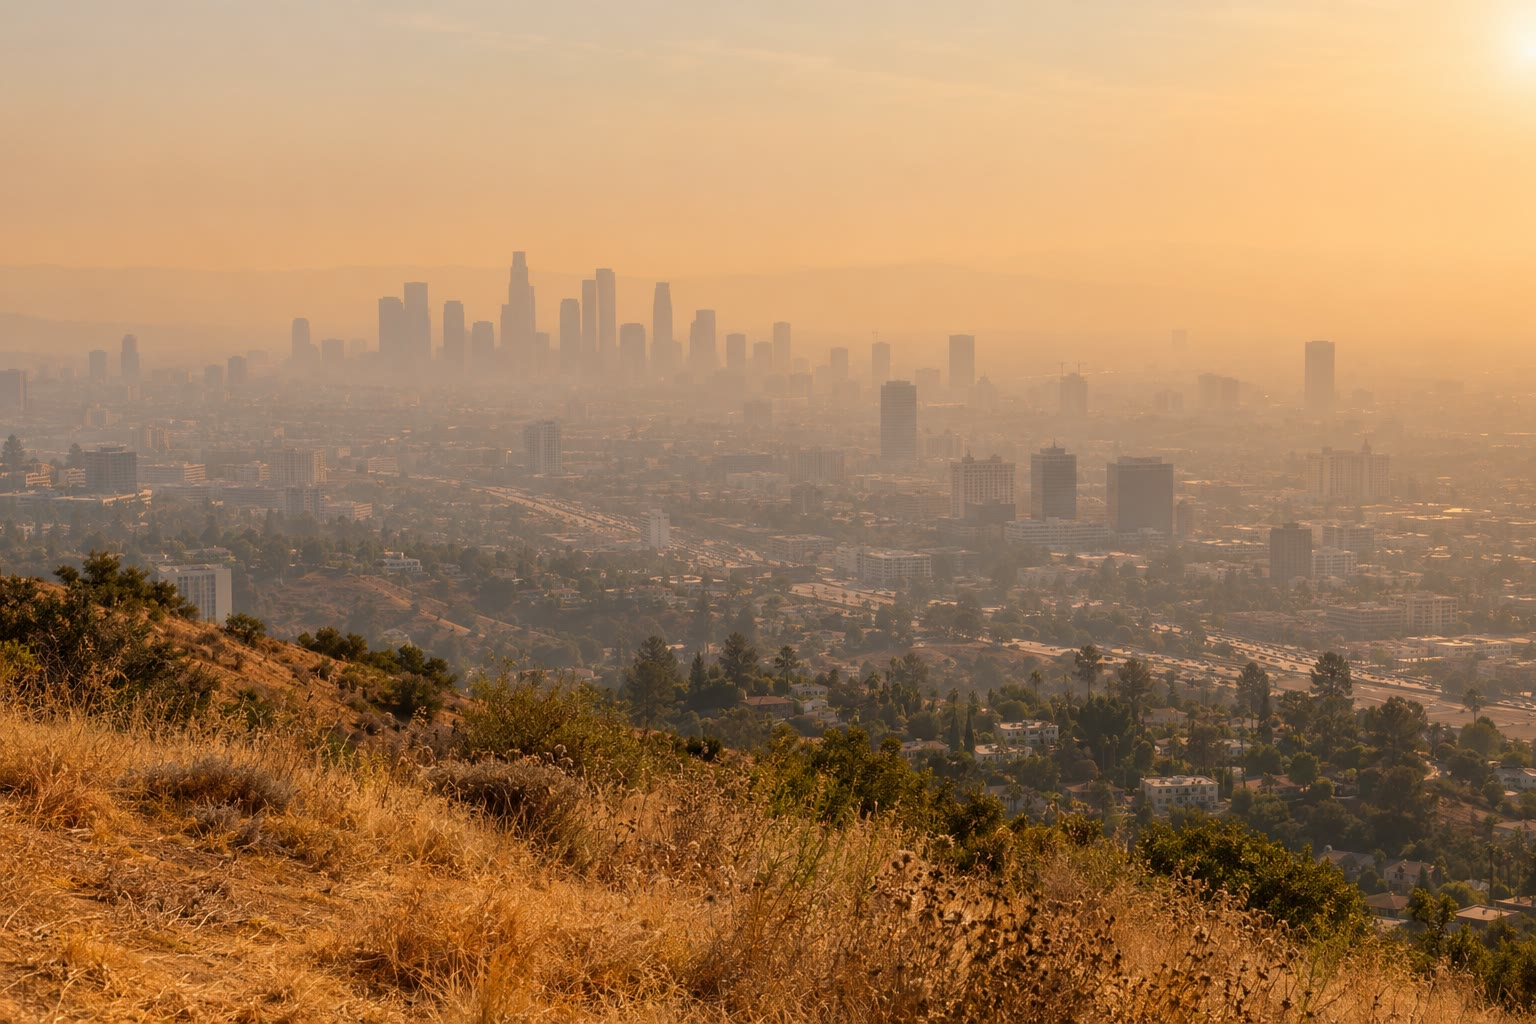
\includegraphics[width=0.6\linewidth]{images/book4/ai/b3-14-smog.jpg}

{\small Une ville sous un \omterm{def:b3:photochemistry:smog}{smog photochimique} par un après-midi chaud. La
teinte brune vient de \ce{NO2}~; l'ozone, qui irrite les poumons, est
invisible.}
\end{omfigure}

\begin{omfigure}
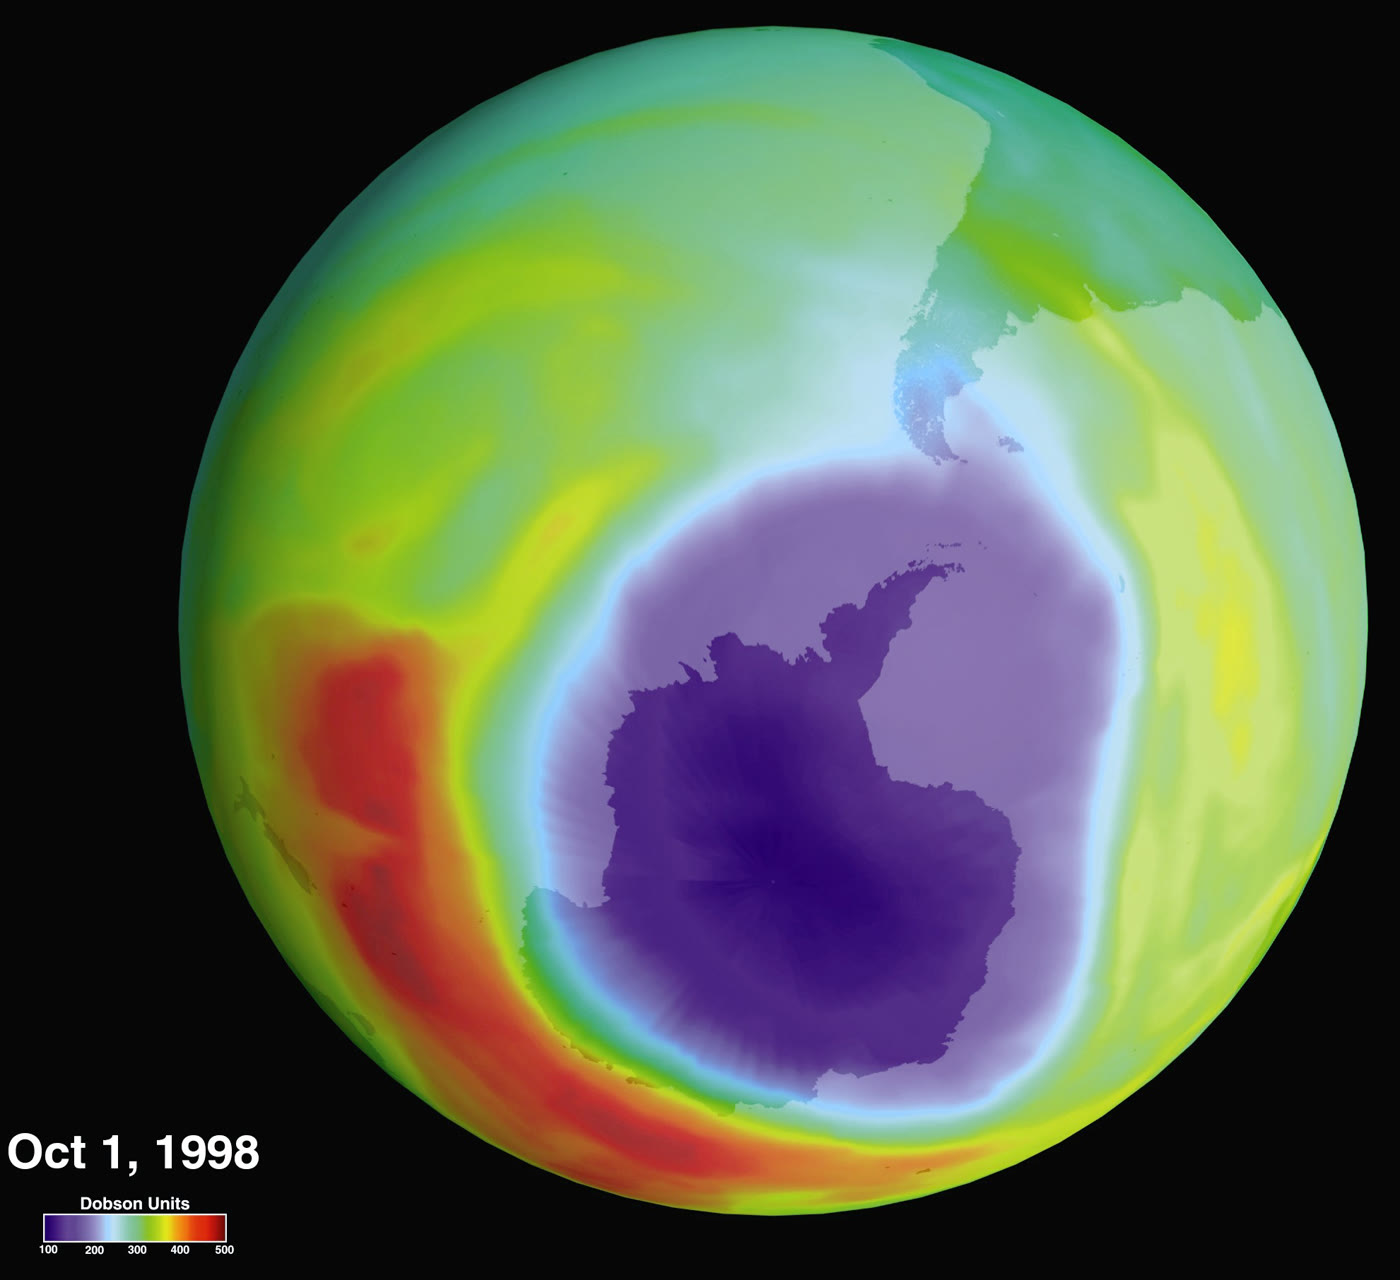
\includegraphics[width=0.5\linewidth]{images/book4/ozone-hole.jpg}

{\small La colonne d'ozone au-dessus de l'hémisphère sud le 1\textsuperscript{er}
octobre 1998, d'après des mesures satellitaires~: le trou de la \omterm{def:b3:photochemistry:chapman}{couche
d'ozone} au-dessus de l'Antarctique (en violet) descend à environ
100 unités Dobson, contre environ 300 ailleurs.}
\end{omfigure}

\begin{inthelab}[Un photoréacteur]
Une lampe à vapeur de mercure moyenne pression, refroidie dans une
chemise de quartz, est placée au centre du réacteur~; un manchon filtrant
en verre élimine les longueurs d'onde inférieures à environ
\qty{300}{nm}, qui détruiraient les produits. La solution est désoxygénée
par un courant de diazote (le dioxygène désactive les triplets) et
agitée. Le réacteur entier est capoté~: la lampe émet un rayonnement
ultraviolet nocif pour les yeux et la peau, et on ne la regarde jamais,
même brièvement.
\end{inthelab}

\begin{safety}{\ghs[0.8cm]{GHS08}\ghs[0.8cm]{GHS09}}
% ledger: ghs4:benzophenone
Benzophénone, sensibilisateur courant et réactif de la photoréduction~:
susceptible de provoquer le cancer, peut endommager des organes après
une exposition prolongée, toxique pour les organismes aquatiques. Pesée et
manipulée avec des gants~; les résidus vont aux déchets organiques.
\end{safety}

\begin{history}[La photochimie de l'avenir, et le trou dans le ciel]
En 1912, Giacomo Ciamician, à Bologne, se demanda si l'industrie ne
pourrait pas un jour fonctionner à la lumière du Soleil, comme les
plantes, plutôt qu'au charbon~; il avait passé des années à exposer au
Soleil des ballons de composés organiques sur le toit de son
laboratoire. En 1985, trois scientifiques travaillant dans une station
de recherche antarctique rapportèrent que la colonne d'ozone printanière
au-dessus d'elle diminuait fortement depuis la fin des années
1970.
Le trou de la \omterm{def:b3:photochemistry:chapman}{couche d'ozone}, expliqué en quelques années par la chimie
de ce chapitre, conduisit à l'abandon progressif des chlorofluorocarbures.
\end{history}

\section{Exercices}

\begin{exercise}[$\star$]\label{exo:b3:photochemistry:1}
Une lampe délivre \qty{100}{mW} à \qty{365}{nm}. Combien de photons par
seconde, et combien d'einstein par seconde~?
\end{exercise}

\begin{exercise}[$\star$]\label{exo:b3:photochemistry:2}
En \qty{10.0}{min}, une solution qui absorbe \qty{1.00e-7}{einstein.s^{-1}}
transforme
\qty{2.0e-5}{mol} de réactif. Calculer le \omterm{def:b3:electronic-spectroscopy:quantum-yield}{rendement quantique}.
\end{exercise}

\begin{exercise}[$\star$]\label{exo:b3:photochemistry:3}
La réaction photochimique de \ce{H2} avec \ce{Cl2} a des \omterm{def:b3:electronic-spectroscopy:quantum-yield}{rendements
quantiques} atteignant $10^4$ et plus. Que montre ce fait~? Écrire les
étapes de propagation.
\end{exercise}

\begin{exercise}[$\star$]\label{exo:b3:photochemistry:4}
% ledger: janaf:O.dfH0, janaf:O3.dfH0
À partir des enthalpies de formation à 0 K de O (\qty{246.79}{kJ/mol}) et
de \ce{O3}
(\qty{145.35}{kJ/mol}), calculer les plus grandes longueurs d'onde
capables de dissocier \ce{O2} en deux atomes et \ce{O3} en \ce{O2} et O.
\end{exercise}

\begin{exercise}[$\star\star$]\label{exo:b3:photochemistry:5}
Un photocommutateur a, à \qty{365}{nm}, $\varepsilon_E = 22\,000$ et
$\varepsilon_Z = 1500$ \unit{L.mol^{-1}.cm^{-1}}, avec
$\Phi_{E\to Z} = 0.11$ et $\Phi_{Z\to E} = 0.40$ (données de l'exercice).
Calculer la composition photostationnaire.
\end{exercise}

\begin{exercise}[$\star\star$]\label{exo:b3:photochemistry:6}
Donner les produits de la \omterm{def:b3:photochemistry:norrish}{réaction de Norrish de type II} de
l'hexan-2-one, et expliquer pourquoi la pentan-2-one donne de l'éthène
plutôt que du propène.
\end{exercise}

\begin{exercise}[$\star\star$]\label{exo:b3:photochemistry:7}
Un accepteur a une énergie triplet de \qty{250}{kJ/mol}. Parmi trois
sensibilisateurs candidats d'énergies triplet 289, 253 et
\qty{236}{kJ/mol} (données de l'exercice), lequel transfère
efficacement~? Estimer la constante d'équilibre du transfert pour chacun
à \qty{298}{K}.
\end{exercise}

\begin{exercise}[$\star\star$]\label{exo:b3:photochemistry:8}
% ledger: kin:O+O2+M.k0, kin:O+O2+M.n
À \qty{230}{K}, avec $[\mathrm M] = \qty{4.0e17}{cm^{-3}}$, $[\ce{O2}] = 0.21[\mathrm M]$ et $j_3 = \qty{1.0e-3}{s^{-1}}$,
calculer $k_2$ et le rapport stationnaire $[\ce{O}]/[\ce{O3}]$.
\end{exercise}

\begin{exercise}[$\star\star$]\label{exo:b3:photochemistry:9}
% ledger: kin:Cl+O3.A, kin:Cl+O3.EaR, kin:Cl+CH4.A, kin:Cl+CH4.EaR
À \qty{230}{K}, calculer les constantes de vitesse de $\ce{Cl + O3}$ et de
$\ce{Cl + CH4}$, et la probabilité qu'un atome Cl rencontre \ce{O3}
plutôt que \ce{CH4} quand $[\ce{O3}] = \qty{5.7e12}{cm^{-3}}$
et $[\ce{CH4}] = \qty{4.0e11}{cm^{-3}}$.
\end{exercise}

\begin{exercise}[$\star\star\star$]\label{exo:b3:photochemistry:10}
% ledger: kin:NO+O3.A, kin:NO+O3.EaR
À midi dans une ville, $[\ce{NO2}]/[\ce{NO}] = 1.5$ et $j_{\ce{NO2}} = \qty{8.0e-3}{s^{-1}}$.
Calculer l'ozone photostationnaire à \qty{298}{K} en molécules par
\unit{cm^3} et en ppb (air sous \qty{1}{bar}).
Que se passe-t-il la nuit~?
\end{exercise}

\begin{exercise}[$\star\star\star$]\label{exo:b3:photochemistry:11}
Une solution de \qty{3.0}{mL}, d'absorbance 0.50 à \qty{313}{nm}, reçoit
\qty{50}{mW} de lumière à cette longueur d'onde~; la réaction a
$\Phi = 0.25$. Calculer la vitesse initiale en
\unit{mol.L^{-1}.s^{-1}}.
\end{exercise}

\begin{exercise}[$\star\star\star$]\label{exo:b3:photochemistry:12}
Un actinomètre au ferrioxalate, de \omterm{def:b3:electronic-spectroscopy:quantum-yield}{rendement quantique} 1.25 à
\qty{365}{nm} (données de l'exercice) et à absorption totale, forme
\qty{3.0e-6}{mol} de Fe(II) en \qty{60}{s}.
Calculer le \omterm{def:b3:photochemistry:photon-flux}{flux de photons}. Pourquoi la conversion doit-elle rester
faible~?
\end{exercise}

\section{Problème~: faire et défaire la couche d'ozone}

\begin{problem}[{Problème du week-end --- faire et défaire la couche
d'ozone~: seuils photoniques, état stationnaire de Chapman avec des
constantes de vitesse évaluées, cycle du chlore, et réservoirs qui
l'arrêtent}]
\label{pb:b3:photochemistry:1}
% ledger: janaf:O.dfH0, janaf:O3.dfH0, kin:O+O2+M.k0, kin:O+O2+M.n, kin:O+O3.A, kin:O+O3.EaR, kin:Cl+O3.A, kin:Cl+O3.EaR, kin:O+ClO.A, kin:O+ClO.EaR, kin:Cl+CH4.A, kin:Cl+CH4.EaR, kin:ClO+NO2+M.k0, kin:ClO+NO2+M.n, kin:ClO+NO2+M.kinf, kin:ClO+NO2+M.Fc, oz:column.mean, oz:column.hole
Un modèle de la stratosphère vers \qty{30}{km} (données du problème)~:
$T = \qty{230}{K}$, $[\mathrm M] =
\qty{4.0e17}{cm^{-3}}$, $[\ce{O2}] = 0.21[\mathrm M]$, \omterm{def:b3:photochemistry:photolysis}{constantes de vitesse de photolyse} $j_1 = \qty{1.0e-11}{s^{-1}}$ (\ce{O2})
et $j_3 = \qty{1.0e-3}{s^{-1}}$ (\ce{O3}), $[\ce{CH4}] = \qty{4.0e11}{cm^{-3}}$, $[\ce{NO2}] = \qty{1.0e9}{cm^{-3}}$.
Constantes de vitesse évaluées (\unit{cm^3.s^{-1}}, ou \unit{cm^6.s^{-1}}
pour $k_2$, les concentrations étant comptées par \unit{cm^3})~:
$k_2 = \num{6.0e-34}(T/300)^{-2.6}$~; $k_4 = \num{8.0e-12}\eu^{-2060/T}$~; Cl + \ce{O3}~: $\num{2.8e-11}\eu^{-250/T}$~;
O + ClO~: $\num{2.5e-11}\eu^{110/T}$~; Cl + \ce{CH4}~: $\num{6.6e-12}\eu^{-1240/T}$~; ClO + \ce{NO2} + M~: $\num{1.41e-13}$ dans
ces conditions.

\medskip\noindent\textbf{Partie I --- Seuils photoniques.}
\begin{enumerate}
  \item Calculer $D_0(\ce{O2})$ à partir de $\Delta_fH^\circ_0(\ce{O}) = \qty{246.79}{kJ/mol}$.
  \item En déduire la plus grande longueur d'onde qui dissocie \ce{O2}.
  \item Calculer l'énergie de $\ce{O3 -> O2 + O}$
        ($\Delta_fH^\circ_0(\ce{O3}) = \qty{145.35}{kJ/mol}$) et sa
        longueur d'onde seuil.
  \item La lumière visible pourrait donc dissocier l'ozone~; pourquoi
        est-ce l'absorption ultraviolette de l'ozone qui importe pour la
        vie~?
  \item Pourquoi \ce{O2} n'est-il photolysé qu'en haute altitude~?
\end{enumerate}

\medskip\noindent\textbf{Partie II --- L'état stationnaire de Chapman.}
\begin{enumerate}[resume]
  \item Écrire les quatre étapes de Chapman.
  \item Calculer $k_2$ et $k_2[\mathrm M]$ à \qty{230}{K}.
  \item Calculer $k_4$.
  \item Calculer $[\ce{O}]/[\ce{O3}]$.
  \item Montrer que $[\ce{O3}] = [\ce{O2}]\sqrt{j_1k_2[\mathrm M]/(j_3k_4)}$.
  \item Calculer $[\ce{O3}]$ et sa fraction molaire.
  \item Calculer $[\ce{O}]$.
  \item L'ozone observé est inférieur à cette valeur. Pourquoi~?
\end{enumerate}

\medskip\noindent\textbf{Partie III --- Le cycle du chlore.}
\begin{enumerate}[resume]
  \item Écrire le cycle et sa réaction bilan.
  \item Calculer la durée de vie d'un atome Cl vis-à-vis de \ce{O3}.
  \item Calculer la durée de vie de ClO vis-à-vis de O.
  \item En déduire le rapport stationnaire $[\ce{ClO}]/[\ce{Cl}]$.
  \item Avec $[\ce{Cl}] + [\ce{ClO}] = \qty{1.0e7}{cm^{-3}}$, comparer la
        vitesse de destruction de l'oxygène impair par le cycle à celle de
        l'étape de Chapman $\ce{O + O3}$.
  \item Quelle étape limite le cycle~?
\end{enumerate}

\medskip\noindent\textbf{Partie IV --- Les réservoirs.}
\begin{enumerate}[resume]
  \item Calculer la probabilité qu'un atome Cl réagisse avec \ce{O3}
        plutôt qu'avec
        \ce{CH4}.
  \item Calculer la probabilité que ClO réagisse avec O plutôt qu'avec
        \ce{NO2}.
  \item En déduire la probabilité $p$ qu'un tour du cycle soit achevé.
  \item En déduire le nombre moyen de tours avant la capture du chlore.
  \item Expliquer comment les nuages stratosphériques polaires allongent
        la chaîne.
  \item Énoncer le résultat~: le nombre de molécules d'ozone qu'un atome
        de chlore détruit, dans ce modèle, avant d'être capturé dans un
        réservoir.
\end{enumerate}
\end{problem}
